% Fermion pair production: cross-validation and numerical error analysis.
\documentclass[11pt,a4paper]{article}
\usepackage[margin=25mm]{geometry}
\usepackage[numbers]{natbib}
\usepackage{amsmath,amssymb,bm}
\usepackage{graphicx,booktabs}
\usepackage{xurl}
\usepackage{placeins}
\usepackage[colorlinks=true,allcolors=blue]{hyperref}
\setlength{\emergencystretch}{1em}
\newcommand{\sech}{\operatorname{sech}}
\hypersetup{pdftitle={Fermion pair production in pulsed electric fields: cross-validation of Dirac and quantum-kinetic calculations},pdfauthor={Othman H. Y. Zalloum},pdfsubject={Fermion pair production in pulsed electric fields},pdfkeywords={fermion pair production, pulsed electric fields, Dirac equation, quantum kinetic theory, numerical convergence}}
\title{Fermion pair production in pulsed electric fields: cross-validation of Dirac and quantum-kinetic calculations}
\author{Othman H. Y. Zalloum\\[3pt]
\small Department of Applied Mathematics and Physics\\
\small Palestine Polytechnic University, Hebron, Palestine\\[3pt]
\small Correspondence: \href{mailto:ozalloum@ppu.edu}{ozalloum@ppu.edu}\\
\small ORCID: \href{https://orcid.org/0000-0001-7282-1332}{0000-0001-7282-1332}}
\date{}
\begin{document}
\maketitle
\begin{abstract}
Reliable fermion pair-production spectra in pulsed electric fields require control of time integration, finite pulse windows and momentum discretization. We compare direct Dirac-mode evolution with the equivalent quantum-kinetic equations for prescribed, spatially homogeneous fields in one spatial dimension. Both formulations use a common instantaneous-vacuum convention and are tested against the exact asymptotic Sauter spectrum. For the reference pulse, their maximum absolute occupation errors on 41 momentum modes are below $8\times10^{-13}$; increasing the integration half-width from six to twelve pulse durations reduces the zero-momentum discrepancy by more than five orders of magnitude. A separated two-pulse field gives agreement between formulations within $1.18\times10^{-13}$. An additional set of 1,962 mode evaluations tests integration controls, endpoints, pulse parameters, a Gaussian profile and momentum-integrated densities. Across nine Sauter parameter pairs, the maximum absolute occupation error at refined settings is $4.58\times10^{-15}$. Grid and domain refinements satisfy a prescribed $10^{-4}$ relative density criterion. These results distinguish agreement between state representations from convergence to asymptotic observables: small conservation errors and agreement between solvers do not alone control finite-window or momentum-domain bias. The accompanying implementation makes the equations, numerical conventions and validation procedure reproducible for the tested homogeneous-field models.
\end{abstract}

\noindent\textbf{Keywords:} fermion pair production, pulsed electric fields, Dirac equation, quantum kinetic theory, numerical convergence.

\section{Introduction}

Pair creation by an electric field connects the vacuum structure of quantum electrodynamics with nonequilibrium particle dynamics. Foundational treatments established vacuum polarization, transmission between Dirac states and pair production in constant or alternating backgrounds \cite{EulerHeisenberg1936,Sauter1931,Schwinger1951,BrezinItzykson1970}. Subsequent mean-field and kinetic approaches described the evolution of particle occupations, including Pauli blocking and memory effects \cite{Kluger1991,Kluger1992,Kluger1998,Schmidt1998,Schmidt1999}.

For a time-dependent field, the final momentum spectrum depends on the pulse history. The temporal Sauter pulse provides an exact reference for testing numerical descriptions, while kinetic, scattering and Wigner formulations offer complementary representations of the same production process \cite{Dumlu2009,Hebenstreit2010,Fedotov2011,Huet2014}. Short pulses, subcycle structure and superposed time scales can modify the spectrum substantially \cite{Hebenstreit2008,Schutzhold2008,Hebenstreit2009}. Interference in temporally structured backgrounds has also been studied using semiclassical and other approaches \cite{DumluDunne2010,DumluDunne2011a,DumluDunne2011b,Akkermans2012,Li2014}. Resolving such spectra numerically requires a specified momentum convention, a consistent definition of the initial vacuum and final occupation, and convergence checks on the quantities of physical interest.

The numerical question addressed here is how to distinguish agreement between two equivalent evolution equations from accuracy of the resulting asymptotic spectrum and integrated density. A calculation can preserve its norm or kinetic invariant while retaining a bias from finite initialization and measurement times. Two solvers can also agree on a finite momentum grid while omitting a contribution to the density outside that grid. These issues call for separate tests of state evolution, temporal endpoints and momentum integration.

We compare a two-component Dirac equation with the full auxiliary-variable quantum-kinetic system under identical prescribed fields. The single Sauter pulse supplies an external benchmark; a separated two-pulse field and a Gaussian profile test agreement beyond that benchmark. Tolerance and step-cap refinements are distinguished from pulse-window, momentum-spacing and momentum-domain refinements. The contribution is a reproducible numerical assessment of these established formulations, with explicit conventions and quantified errors for the reported cases. The accompanying code supplies the implementation and reproduction materials. Section~\ref{sec:model} defines the physical model, Section~\ref{sec:software} specifies the numerical protocol, and Section~\ref{sec:results} presents the comparisons. Section~\ref{sec:discussion} discusses their implications and limits. Detailed reproduction instructions accompany the computational materials.

\section{Physical model and observables}
\label{sec:model}

We consider a prescribed electric field in one spatial dimension, neglecting back-reaction and collisions. Spatial homogeneity allows each canonical momentum mode to evolve independently. Natural units, $\hbar=c=1$, and temporal gauge, $A^0=0$, are used throughout. With positive charge magnitude $q$, the kinetic momentum is
\begin{equation}
  \pi_p(t)=p-qA(t), \qquad E(t)=-\dot A(t).
  \label{eq:kinetic}
\end{equation}
The reference field is the temporal Sauter pulse,
\begin{align}
  E(t)&=E_0\sech^2\!\left(\frac{t-t_c}{\tau}\right),\nonumber\\
  A(t)&=-E_0\tau\tanh\!\left(\frac{t-t_c}{\tau}\right),
  \label{eq:sauter}
\end{align}
where $E_0\geq0$ and $\tau>0$. Separated pulses are constructed by summing both fields and potentials, preserving $E=-\dot A$. All numerical cases below set $m=q=1$; momenta, times and field strengths are consequently given in units of $m$, $m^{-1}$ and $m^2/q$, respectively. The spectra are plotted against canonical momentum in the specified gauge. The corresponding final kinetic momentum is $p-qA(t_f)$.

\subsection{Dirac-mode evolution and particle occupation}

For each momentum, the two-component spinor obeys
\begin{equation}
  H_p(t)=\pi_p(t)\sigma_1+m\sigma_3, \qquad
  i\partial_t\psi_p(t)=H_p(t)\psi_p(t),
  \label{eq:dirac}
\end{equation}
where $\sigma_i$ are Pauli matrices and $m>0$. Let $u_{p,\pm}(t)$ be normalized instantaneous eigenvectors with energies $\pm\omega_p(t)$, where $\omega_p(t)=\sqrt{m^2+\pi_p(t)^2}$. The finite-time initial vacuum is specified by $\psi_p(t_i)=u_{p,-}(t_i)$, and the occupation at $t_f$ is
\begin{equation}
  f_p^{\mathrm D}(t_f)=\left|u_{p,+}^{\dagger}(t_f)\psi_p(t_f)\right|^2.
  \label{eq:occupation}
\end{equation}
As the endpoints recede into the pulse tails, this projection approaches the asymptotic in/out definition. Exact evolution preserves $\psi_p^\dagger\psi_p=1$; its numerical deviation is monitored independently of the occupation.

\subsection{Quantum-kinetic evolution}

The quantum-kinetic equations (QKE) evolve an occupation $f_p^{\mathrm K}$ and two auxiliary functions $u_p,v_p$. With $W_p(t)=qE(t)m/\omega_p(t)^2$, they read
\begin{align}
  \dot f_p^{\mathrm K} &= \frac{1}{2}W_p u_p, \nonumber\\
  \dot u_p &= W_p(1-2f_p^{\mathrm K})-2\omega_p v_p, \label{eq:qke}\\
  \dot v_p &= 2\omega_p u_p. \nonumber
\end{align}
The initial state $(f_p^{\mathrm K},u_p,v_p)=(0,0,0)$ at $t_i$ represents the same instantaneous vacuum as the Dirac initialization. Although local in these three variables, the system represents the non-Markovian kinetic evolution \cite{Schmidt1998,Dumlu2009}. It preserves the Bloch-vector invariant
\begin{equation}
  I_p=(1-2f_p^{\mathrm K})^2+u_p^2+v_p^2=1.
  \label{eq:invariant}
\end{equation}
The finite-time occupations from Eqs.~\eqref{eq:occupation} and \eqref{eq:qke} are compared at matching endpoints. Their common asymptotic limit is the quantity tested against the exact result below. Superscripts are omitted where a statement applies to either formulation.

\subsection{Exact benchmark and integrated density}

For a single Sauter pulse, define $\lambda=qE_0\tau^2$ and
\begin{equation}
  \omega_{\pm}=\sqrt{m^2+(p\pm qE_0\tau)^2}.
\end{equation}
The asymptotic occupation per fermionic mode is \cite{Hebenstreit2010}
\begin{equation}
  f_p^{\mathrm{exact}}=
  \frac{\cosh(2\pi\lambda)-
  \cosh\!\left[\pi\tau(\omega_+-\omega_-)\right]}
  {2\sinh(\pi\tau\omega_+)\sinh(\pi\tau\omega_-)}.
  \label{eq:exact}
\end{equation}
No additional spin-degeneracy factor is included. The spin-summed distribution in Eq.~(99) of Ref.~\cite{Hebenstreit2010}, at zero transverse momentum, is twice the per-mode occupation used here. The implementation evaluates an algebraically equivalent logarithmic expression to reduce overflow of the hyperbolic functions. This does not guarantee relative accuracy at arbitrarily small occupations. Equation~\eqref{eq:exact} is applied only to a single Sauter pulse.

The momentum-integrated observable is the density for one mode species in one spatial dimension,
\begin{equation}
  n_{1\mathrm D}=\int\frac{dp}{2\pi}f_p.
  \label{eq:density}
\end{equation}
It has dimensions of inverse length and is reported in units of $m$. It is not a three-dimensional density. Numerical values use the trapezoidal rule on a finite interval $[-P,P]$; the number of nodes and the interval width are refined separately.

\section{Numerical method and validation protocol}
\label{sec:software}

\subsection{Integration controls and endpoint conventions}

Both initial-value problems use SciPy's DOP853 implementation through \texttt{solve\_ivp}. Unless specified otherwise, the relative and absolute tolerances are $2\times10^{-10}$ and $2\times10^{-12}$. For a single pulse, a dimensionless tail extent $\ell$ gives endpoints $t_i=t_c-\ell\tau$ and $t_f=t_c+\ell\tau$. For a pulse train, the integration interval spans the union of these individual intervals. The default is $\ell=12$. In the single-pulse window scans, $L=\ell\tau$ denotes the physical half-width.

For each mode, 257 equally spaced times in the integration interval are used to estimate the largest instantaneous frequency, $\widehat\omega_{\max}$. The maximum internal step is $c_h/\widehat\omega_{\max}$, with default $c_h=0.18$. This sampled cap limits steps on the estimated oscillation scale; it is an empirical control rather than a rigorous frequency bound for arbitrary pulse shapes. Changes in tolerance and $c_h$ are therefore tested independently.

The Dirac and kinetic state equations are implemented separately but use the same time integrator, interval, tolerances and cap rule. Their agreement tests consistency of the state representations, while the exact Sauter result and independent refinement studies test errors that can be common to both. Pulse objects must supply consistent $E(t)$ and $A(t)$ and suitable endpoints. The software interface does not enforce those physical conditions automatically.

The calculations were performed in Python using NumPy and SciPy. Source code, reproduction instructions, software requirements and execution checks are provided in the accompanying computational archive, including its \texttt{REPRODUCIBILITY.txt} notes.

\subsection{Error measures and acceptance criteria}

For formulation $X\in\{\mathrm D,\mathrm K\}$, the absolute Sauter benchmark error and the difference between formulations are
\begin{align}
  \epsilon_p^X&=\left|f_p^X(t_f)-f_p^{\mathrm{exact}}\right|,\nonumber\\
  \delta_p&=\left|f_p^{\mathrm D}(t_f)-f_p^{\mathrm K}(t_f)\right|.
  \label{eq:errors}
\end{align}
The benchmark error includes the effects of finite endpoints, numerical integration and floating-point arithmetic. Final-time conservation diagnostics are
\begin{equation}
  \eta_p^{\mathrm D}=|\psi_p^\dagger\psi_p-1|,\qquad
  \eta_p^{\mathrm K}=|I_p-1|.
  \label{eq:diagnostics}
\end{equation}
These are endpoint diagnostics, not maxima along a trajectory or bounds on $\epsilon_p^X$. For density refinement, successive estimates are compared using $|n_{\mathrm{new}}-n_{\mathrm{old}}|/|n_{\mathrm{new}}|$.

The additional validation studies comprise 1,962 individual mode evaluations: 180 for integration controls, 60 for endpoints, 234 for Sauter parameter coverage, 40 for a Gaussian profile, 962 for momentum integration and 486 for density sensitivity to time-evolution controls. These counts are separate from the illustrative spectra and the momentum--window map. All reported evaluations completed without integration failures. The recorded protocol requires occupation differences below $10^{-10}$, relative Sauter errors below $10^{-5}$ for exact occupations at least $10^{-10}$, successive relative density changes below $10^{-4}$, and occupations within $[0,1]$ to a tolerance of $10^{-10}$. These are empirical acceptance criteria. Unsuccessful integrations are retained by the scripts rather than discarded. The reference spectrum below also reports relative errors using its explicitly stated $10^{-12}$ occupation threshold.

\FloatBarrier
\section{Results}
\label{sec:results}

\subsection{Sauter spectrum and asymptotic benchmark}

The reference pulse has $E_0=0.3$, $\tau=2$ and $t_c=0$, with 41 equally spaced momenta on $[-1.5,1.5]$. Figure~\ref{fig:sauter} compares both formulations at $\ell=12$ with the exact asymptotic spectrum. The largest absolute errors are $7.48\times10^{-13}$ for Dirac evolution and $7.54\times10^{-13}$ for QKE. Over modes with $f_p^{\mathrm{exact}}>10^{-12}$, each formulation has maximum relative error $1.68\times10^{-8}$. The maximum final-time norm and kinetic-invariant errors across the grid are $6.24\times10^{-13}$ and $9.13\times10^{-13}$, respectively.

\begin{figure}[htbp]
  \centering
  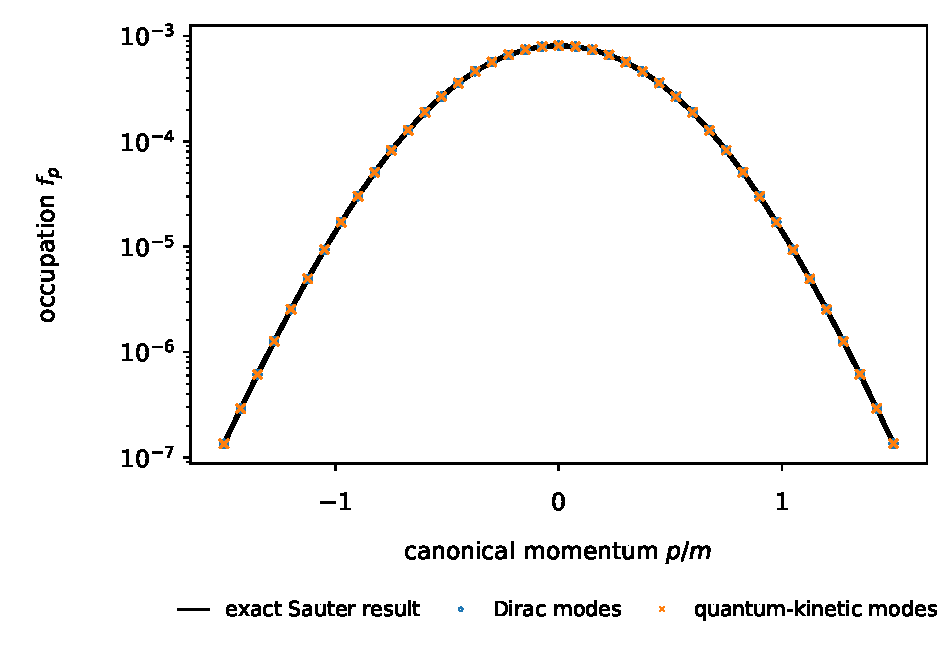
\includegraphics[width=0.78\linewidth]{figure1_sauter_validation.pdf}
  \caption{Single-pulse occupation spectrum for $E_0=0.3$, $\tau=2$, $t_c=0$, and $m=q=1$, evaluated at 41 equally spaced canonical momenta in $[-1.5,1.5]$. The black line is the exact asymptotic Sauter result; circles and crosses denote Dirac and quantum-kinetic modes integrated over $[-12\tau,12\tau]$. The numerical results lie on the exact curve at this resolution. The vertical axis is logarithmic; markers represent deterministic calculations, with no statistical error bars.}
  \label{fig:sauter}
\end{figure}

At zero momentum, $f_0^{\mathrm{exact}}=8.11991615993\times10^{-4}$. Table~\ref{tab:tail} shows that increasing $L/\tau$ from 6 to 12 at fixed solver controls reduces the absolute discrepancy by more than five orders of magnitude. At $L/\tau=14$, the discrepancies are of order $10^{-14}$. The close correspondence of the two error sequences illustrates a shared sensitivity to finite endpoints. This scan alone does not isolate residual tail error from integration error and roundoff; the separate refinements in Section~\ref{sec:refinement} address that distinction.

\begin{table}[tp]
  \centering
  \small
  \caption{Finite-window convergence at $p=0$ for $E_0=0.3$, $\tau=2$, $t_c=0$, and $m=q=1$. Endpoints are $t_i=-L$, $t_f=L$. Both solvers use relative tolerance $2\times10^{-10}$, absolute tolerance $2\times10^{-12}$, and the step cap in Section~\ref{sec:software}. Errors are absolute differences from Eq.~\eqref{eq:exact}; numerical tolerances are held fixed as $L$ varies.}
  \label{tab:tail}
  \begin{tabular}{rrrr}
    \toprule
    Tail half-width $L/\tau$ & Exact & Dirac absolute error & QKE absolute error\\
    \midrule
    6  & $8.11991615993\times10^{-4}$ & $1.1762\times10^{-7}$ & $1.1762\times10^{-7}$\\
    8  & $8.11991615993\times10^{-4}$ & $2.1989\times10^{-9}$ & $2.1989\times10^{-9}$\\
    10 & $8.11991615993\times10^{-4}$ & $4.0728\times10^{-11}$ & $4.0721\times10^{-11}$\\
    12 & $8.11991615993\times10^{-4}$ & $7.4813\times10^{-13}$ & $7.5435\times10^{-13}$\\
    14 & $8.11991615993\times10^{-4}$ & $1.2825\times10^{-14}$ & $6.7149\times10^{-15}$\\
    \bottomrule
  \end{tabular}
\end{table}

\subsection{Separated-pulse spectrum}

The second field is a sum of two same-polarity Sauter pulses, each with $E_0=0.3$ and $\tau=1.1$, centred at $t_c=\pm3.5$. With $\ell=12$, the common integration interval is $[-16.7,16.7]$. Figure~\ref{fig:double} displays 41 equally spaced momenta on $[-1.8,1.8]$. Both formulations resolve the central maximum and its adjacent shoulders and modulations; their largest absolute occupation difference is $1.18\times10^{-13}$. This comparison extends the numerical consistency check to a field for which no closed-form spectrum is used in the study.

\begin{figure}[htbp]
  \centering
  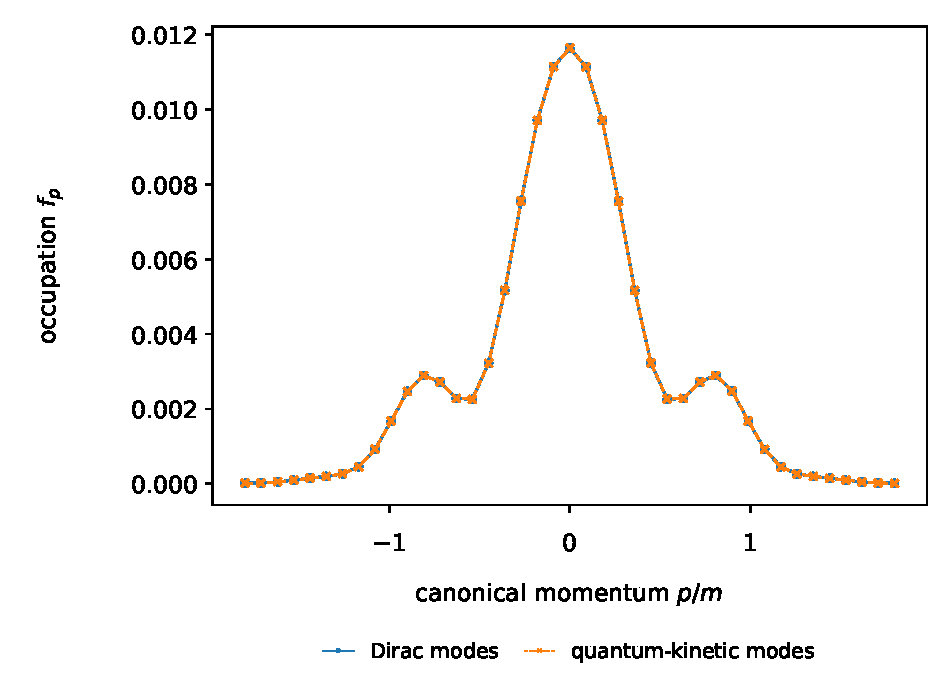
\includegraphics[width=0.78\linewidth]{figure2_double_pulse.pdf}
  \caption{Occupation spectrum for two separated, same-polarity Sauter pulses, each with $E_0=0.3$ and $\tau=1.1$, centred at $t_c=\pm3.5$, with $m=q=1$. Circles with a solid line and crosses with a dashed line denote Dirac and quantum-kinetic calculations on 41 equally spaced canonical momenta in $[-1.8,1.8]$. Endpoints are $t_i=-16.7$, $t_f=16.7$. Lines join computed modes; no analytic curve is supplied for this case.}
  \label{fig:double}
\end{figure}

The agreement establishes that the displayed structure is reproduced by both state representations at matching numerical settings. Attribution of individual features to a particular interference mechanism would require additional analysis of their dependence on pulse parameters or of the relevant amplitudes and phases. The present calculation does not make that attribution.

On the finite grids in Figures~\ref{fig:sauter} and \ref{fig:double}, trapezoidal integration gives $n_{1\mathrm D}=1.13951\times10^{-4}$ for the exact single-pulse spectrum and $1.69199\times10^{-3}$ for the double-pulse spectrum. Section~\ref{sec:densityvalidation} examines how these estimates change when the momentum spacing and range are refined.

\subsection{Conservation diagnostics and finite-window discrepancy}

Figure~\ref{fig:invariant} shows the final-time kinetic-invariant error over the reference momentum grid. Its maximum is below $10^{-12}$. Conservation provides a check on integration of Eq.~\eqref{eq:qke}, but the invariant does not fix the occupation uniquely: it constrains the combined values of $f_p^{\mathrm K}$, $u_p$ and $v_p$. A small invariant error therefore complements, rather than replaces, an occupation benchmark.

\begin{figure}[htbp]
  \centering
  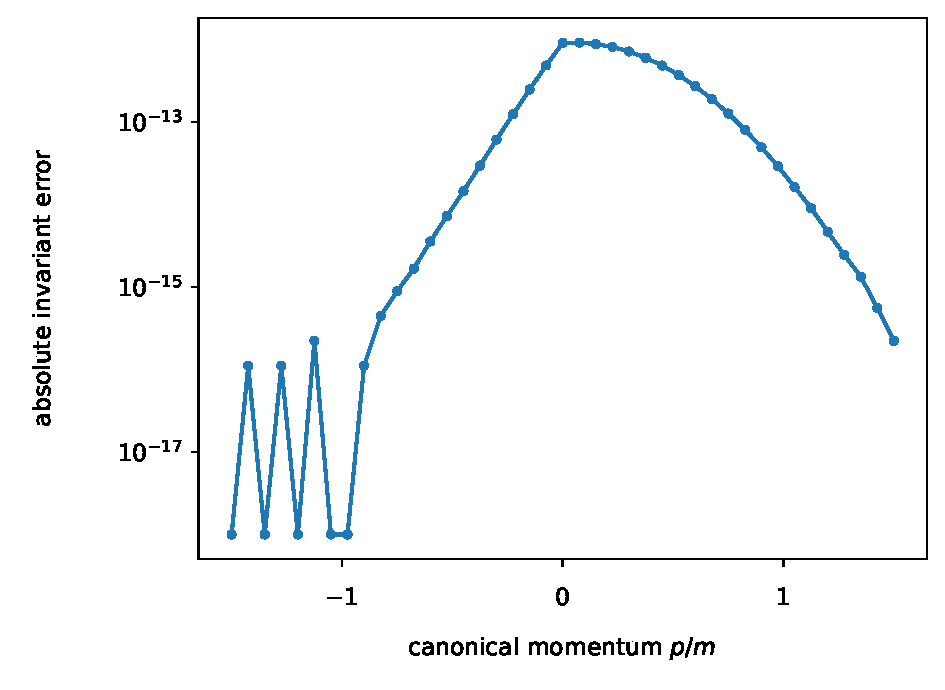
\includegraphics[width=0.78\linewidth]{figure3_qke_invariant.pdf}
  \caption{Final-time quantum-kinetic invariant error $|(1-2f_p)^2+u_p^2+v_p^2-1|$ for the single-pulse setup of Figure~\ref{fig:sauter}. Each marker corresponds to one of 41 momentum modes, evaluated at $t_f=12\tau$; the connecting line guides the eye. Values are plotted on a logarithmic scale with a display floor of $10^{-18}$. The diagnostic measures conservation of the invariant, not occupation error or a maximum over time.}
  \label{fig:invariant}
\end{figure}

Figure~\ref{fig:window-error} extends the endpoint comparison across 41 momenta and six half-widths, $L/\tau=4,6,8,10,12,14$, for the same $E_0=0.3$ and $\tau=2$ pulse. The common colour scale permits direct comparison of absolute discrepancies between the two formulations. The map records momentum dependence as well as convergence with window extent. Its values include finite-window, fixed-tolerance integration and roundoff effects; the smallest discrepancies cannot be identified as pure tail errors. The field remains spatially homogeneous, so the horizontal coordinate is momentum, not position.

\begin{figure}[tp]
  \centering
  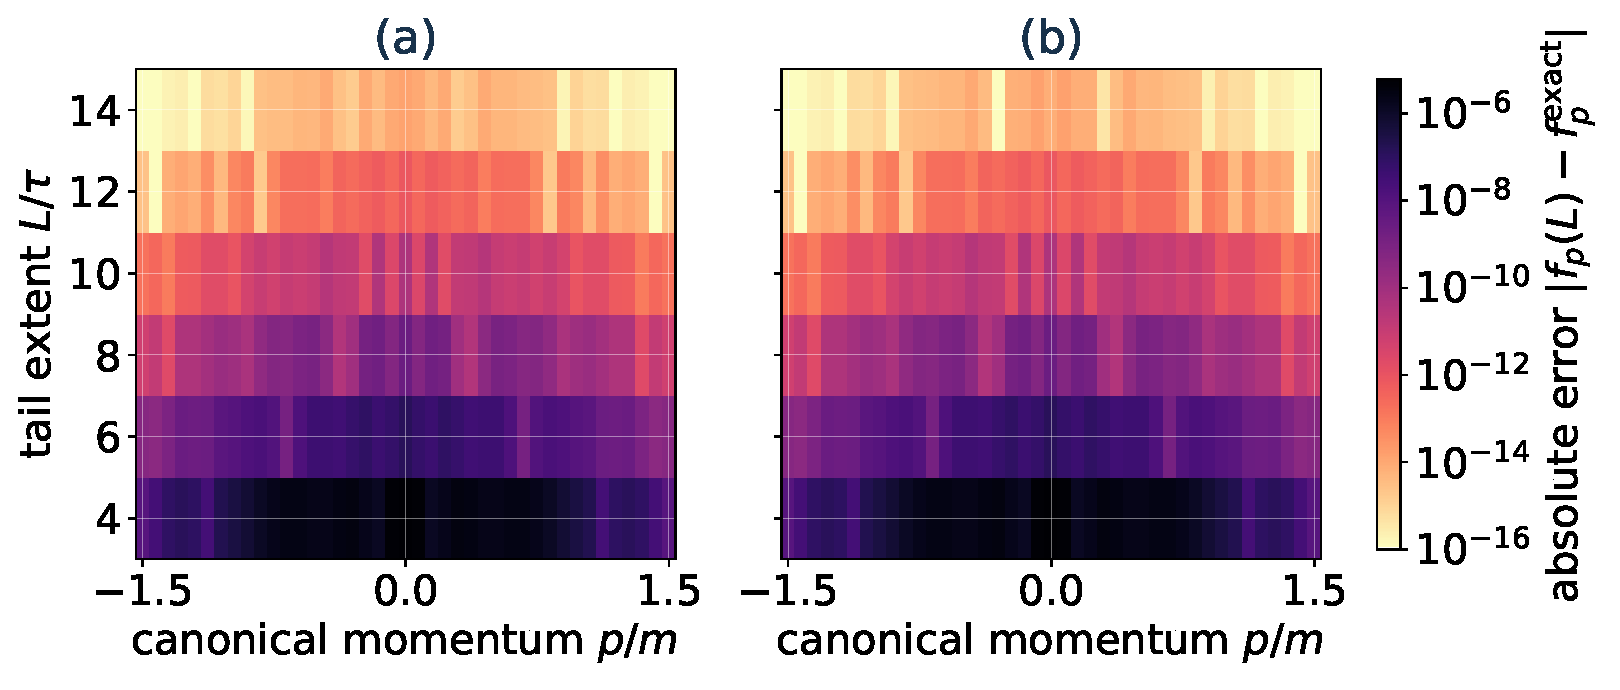
\includegraphics[width=0.94\textwidth]{figure4_sauter_window_error_map.pdf}
  \caption{Absolute finite-window discrepancy $|f_p(L)-f_p^{\mathrm{exact}}|$ from the asymptotic Sauter benchmark: (a) Dirac modes and (b) quantum-kinetic modes, for $E_0=0.3$, $\tau=2$, $t_c=0$, and $m=q=1$. Each panel contains 41 momenta in $[-1.5,1.5]$ and six half-widths $L/\tau=4,6,8,10,12,14$; integration endpoints are $t_c\pm L$. The common logarithmic colour scale uses a display floor of $10^{-16}$ without changing the computed errors. Discrepancies include window, integration, and roundoff effects at fixed tolerances. The horizontal coordinate is canonical momentum, not position.}
  \label{fig:window-error}
\end{figure}

\FloatBarrier
\subsection{Integration and endpoint refinements}
\label{sec:refinement}

At fixed tail extent $\ell=20$, the single- and double-pulse cases are each tested at $p=0,\pm0.75,\pm1.5$. The relative tolerance takes values $2\times10^{-8}$, $2\times10^{-10}$ and $2\times10^{-12}$, with absolute tolerance one hundredth as large. Independently, $c_h$ takes values 0.18, 0.09 and 0.045. Both formulations are run at all combinations, giving 180 evaluations. Relative to the same formulation at the tightest tolerance and cap, the largest absolute occupation difference is $8.46\times10^{-14}$. Refinement differences need not decrease monotonically near floating-point precision. For the double pulse, this comparison uses a refined numerical reference rather than an exact solution.

A separate set of 60 evaluations varies $\ell$ through 12, 16 and 20 at relative tolerance $2\times10^{-12}$ and $c_h=0.045$. Relative to $\ell=20$, the largest occupation differences at $\ell=12$ are $7.48\times10^{-13}$ for the single pulse and $2.59\times10^{-13}$ for the double pulse. At $\ell=16$, they are below $2.51\times10^{-16}$ and $9.37\times10^{-16}$, respectively. Holding the tighter integration controls fixed separates this endpoint-sensitivity test from the preceding fixed-window study.

\subsection{Field strength, duration and pulse profile}

The exact benchmark is tested at all nine combinations of $E_0=0.1,0.3,0.8$ and $\tau=0.5,2,5$. Each pair uses 13 equally spaced momenta on $[-p_{\max},p_{\max}]$, with $p_{\max}=\max(1.5,E_0\tau+2/\tau)$ in the units specified in Section~\ref{sec:model}. The controls are $\ell=20$, relative tolerance $2\times10^{-12}$, absolute tolerance $2\times10^{-14}$ and $c_h=0.09$. Table~\ref{tab:parameter} summarizes the resulting 234 evaluations. The maximum absolute error is $4.58\times10^{-15}$, and the maximum relative error for exact occupations at least $10^{-10}$ is $1.83\times10^{-9}$. No negative occupations or upper-bound violations occur in this sweep. The smallest exact occupation is $7.81\times10^{-19}$; relative accuracy is not asserted at that scale.

\begin{table}[htbp]
\centering\small
\caption{Maximum absolute Sauter occupation error over 13 momenta per parameter pair for $m=q=1$. The field strength and duration use the units defined in Section~\ref{sec:model}; integration settings are specified in the text.}
\label{tab:parameter}
\begin{tabular}{rrrr}\toprule
$E_0$ & $\tau$ & Dirac & QKE\\\midrule
0.1 & 0.5 & $4.84\times10^{-17}$ & $8.19\times10^{-16}$\\
0.1 & 2 & $4.02\times10^{-18}$ & $1.71\times10^{-18}$\\
0.1 & 5 & $8.39\times10^{-20}$ & $4.12\times10^{-19}$\\
0.3 & 0.5 & $9.71\times10^{-17}$ & $2.71\times10^{-15}$\\
0.3 & 2 & $5.43\times10^{-17}$ & $2.76\times10^{-17}$\\
0.3 & 5 & $5.90\times10^{-17}$ & $9.67\times10^{-18}$\\
0.8 & 0.5 & $4.27\times10^{-15}$ & $4.58\times10^{-15}$\\
0.8 & 2 & $6.45\times10^{-16}$ & $1.77\times10^{-16}$\\
0.8 & 5 & $1.54\times10^{-15}$ & $1.42\times10^{-16}$\\
\bottomrule\end{tabular}
\end{table}

A smooth Gaussian field supplies a further comparison beyond the Sauter family,
\begin{align}
E(t)&=0.3\exp[-(t/2)^2],\nonumber\\
A(t)&=-0.3\sqrt{\pi}\,\operatorname{erf}(t/2).
\label{eq:gaussian}
\end{align}
These expressions satisfy $E=-\dot A$. Five momenta ($p=0,\pm0.75,\pm1.5$), two endpoint choices ($|t|=12,16$), two cap coefficients (0.09, 0.045) and both formulations give 40 evaluations at relative tolerance $2\times10^{-12}$. The largest absolute difference between formulations at matching settings is $1.31\times10^{-17}$. This tests consistency for a different smooth profile; no independent exact occupation is used for the Gaussian case.

\subsection{Momentum-integrated density}
\label{sec:densityvalidation}

The QKE density is first evaluated using 41, 81 and 161 nodes on each original momentum interval. The spacing of the 161-node grid is then held fixed while the interval is doubled and tripled, giving 321 and 481 nodes. A nested 481-node grid for each pulse case supplies 962 directly evaluated modes, without imposing spectrum symmetry. All use $\ell=20$, relative tolerance $2\times10^{-12}$, absolute tolerance $2\times10^{-14}$ and $c_h=0.09$.

\begin{table}[htbp]
\centering\small
\caption{Trapezoidal density refinement using QKE. $P$ is the momentum half-width in units of $m$, $N_p$ is the number of nodes, and $n_{1\mathrm D}$ is in units of $m$. Grid spacing is refined at fixed $P$ before extending the domain at fixed spacing.}
\label{tab:density}
\begin{tabular}{lrrr}\toprule
Case & $P$ & $N_p$ & $n_{1\mathrm D}$\\\midrule
Single & 1.5 & 41 & $1.1395114844\times10^{-4}$\\
 & 1.5 & 81 & $1.1395130337\times10^{-4}$\\
 & 1.5 & 161 & $1.1395134244\times10^{-4}$\\
 & 3.0 & 321 & $1.1395539392\times10^{-4}$\\
 & 4.5 & 481 & $1.1395539392\times10^{-4}$\\
Double & 1.8 & 41 & $1.6919881473\times10^{-3}$\\
 & 1.8 & 81 & $1.6919976391\times10^{-3}$\\
 & 1.8 & 161 & $1.6920000711\times10^{-3}$\\
 & 3.6 & 321 & $1.6926588379\times10^{-3}$\\
 & 5.4 & 481 & $1.6926588400\times10^{-3}$\\
\bottomrule\end{tabular}
\end{table}

The final fixed-domain grid refinement changes the single- and double-pulse densities by relative amounts $3.43\times10^{-7}$ and $1.44\times10^{-6}$. However, doubling the momentum interval at that spacing changes the corresponding densities by approximately $3.56\times10^{-5}$ and $3.89\times10^{-4}$, as calculated from Table~\ref{tab:density}. The double-pulse change exceeds the prescribed $10^{-4}$ density criterion despite the much smaller fixed-domain grid change. Momentum-spacing convergence alone is therefore insufficient for this case.

The final extension from twice to three times the original half-width changes the densities by $7.20\times10^{-13}$ and $1.21\times10^{-9}$, respectively. The largest difference between numerical and exact single-pulse densities on identical grids is below $1.71\times10^{-18}$. A further 486 evaluations on 81-node grids vary $\ell=12,16,20$ and halve the cap coefficient at $\ell=20$; the largest relative density change is $4.98\times10^{-11}$. The final grid, domain and time-evolution checks meet the $10^{-4}$ criterion. They provide finite refinement evidence, rather than a rigorous bound on the continuum integral.

\FloatBarrier
\section{Discussion}
\label{sec:discussion}

The comparisons distinguish three questions: whether each state evolution preserves its internal constraints, whether the two representations give the same occupation, and whether that occupation and its momentum integral have converged to the intended observables. These tests have different roles. Norm and invariant conservation examine internal evolution. Agreement between formulations checks their implementation under common conventions. The exact Sauter result additionally tests the asymptotic occupation, while endpoint and momentum refinements address truncations that both solvers can share.

The Sauter window scan illustrates why this distinction matters. At short windows, both formulations give nearly identical absolute errors relative to the asymptotic benchmark. They are initialized in the same finite-time vacuum and projected at the same finite endpoint, so agreement need not imply that pulse-tail effects are negligible. Extending the interval reduces the discrepancy strongly for the reference pulse. The separate integration-control study is needed to assess whether a remaining difference is sensitive to numerical evolution at a fixed interval. Values near machine precision should be interpreted as observed discrepancies for those calculations, not as general accuracy guarantees.

The density study identifies a second, distinct truncation issue. Fine sampling of a restricted momentum interval can stabilize the trapezoidal estimate before the interval captures the relevant spectral tails. For the double pulse, the first domain enlargement changes the density by about $3.9\times10^{-4}$ even after the fixed-domain spacing check has converged much more closely. Separate variation of momentum spacing and range is thus necessary when using spectra to report integrated yields. The converged density estimates and occupation comparisons characterize the numerical cases studied here; differences between the single- and double-pulse yields are not interpreted as enhancement at fixed field energy or fluence.

The assessment uses established pair-production equations and does not propose a new production mechanism or analytic solution. Its physical scope is a prescribed homogeneous field in one spatial dimension, without transverse momentum, spatial gradients, back-reaction, collisions or scalar particles. The finite set of Sauter, separated-pulse and Gaussian cases does not supply a parameter-independent error bound. Much weaker occupations, stronger or longer pulses, sharply structured fields and larger pulse trains require additional checks. For backgrounds without an exact result, comparison with a further independent numerical method would strengthen validation beyond the two state representations studied here. Computational scaling and high-throughput performance are outside the present assessment.

\section{Conclusion}

We have compared Dirac-mode and quantum-kinetic calculations of fermion pair production using a common definition of the finite-time vacuum and final occupation. The reference Sauter spectrum is reproduced with maximum absolute error below $8\times10^{-13}$ at the stated default controls, while nine parameter pairs give a maximum error of $4.58\times10^{-15}$ at refined settings. The separated-pulse spectrum agrees between formulations within $1.18\times10^{-13}$. The additional 1,962 mode evaluations separate integration-control, endpoint, pulse-profile and momentum-integration checks.

The central numerical result is the distinction between consistency of state evolution and convergence of physical observables. In the reported cases, endpoint extension is essential for comparison with an asymptotic spectrum, and domain extension is essential for the double-pulse density even after momentum-spacing refinement. The final density checks meet the prescribed $10^{-4}$ relative criterion. The accompanying implementation provides a reproducible basis for these comparisons and for further validation within the stated homogeneous-field model.

\section*{Data availability}
The source code, detailed execution notes, reproduction and validation scripts, and notebook are available in \texttt{Supplementary\_code.zip} at \url{https://github.com/ozalloum/Fermion-Pair-Production}. These scripts generate the numerical datasets and diagnostics used in this study.

\section*{Declaration of competing interest}
The author declares that there are no known competing financial interests or personal relationships that could have appeared to influence the work reported in this paper.

\FloatBarrier
\begin{thebibliography}{99}
\bibitem{EulerHeisenberg1936}
W. Heisenberg and H. Euler, Folgerungen aus der Diracschen Theorie des Positrons, \textit{Zeitschrift f\"ur Physik} 98 (1936) 714--732. \url{https://doi.org/10.1007/BF01343663}.

\bibitem{Sauter1931}
F. Sauter, \"Uber das Verhalten eines Elektrons im homogenen elektrischen Feld nach der relativistischen Theorie Diracs, \textit{Zeitschrift f\"ur Physik} 69 (1931) 742--764. \url{https://doi.org/10.1007/BF01339461}.

\bibitem{Schwinger1951}
J. Schwinger, On gauge invariance and vacuum polarization, \textit{Physical Review} 82 (1951) 664--679. \url{https://doi.org/10.1103/PhysRev.82.664}.

\bibitem{BrezinItzykson1970}
E. Br\'ezin and C. Itzykson, Pair production in vacuum by an alternating field, \textit{Physical Review D} 2 (1970) 1191--1199. \url{https://doi.org/10.1103/PhysRevD.2.1191}.

\bibitem{Kluger1991}
Y. Kluger, J. M. Eisenberg, B. Svetitsky, F. Cooper, and E. Mottola, Pair production in a strong electric field, \textit{Physical Review Letters} 67 (1991) 2427--2430. \url{https://doi.org/10.1103/PhysRevLett.67.2427}.

\bibitem{Kluger1992}
Y. Kluger, J. M. Eisenberg, B. Svetitsky, F. Cooper, and E. Mottola, Fermion pair production in a strong electric field, \textit{Physical Review D} 45 (1992) 4659. \url{https://doi.org/10.1103/PhysRevD.45.4659}.

\bibitem{Kluger1998}
Y. Kluger, E. Mottola, and J. M. Eisenberg, Quantum Vlasov equation and its Markov limit, \textit{Physical Review D} 58 (1998) 125015. \url{https://doi.org/10.1103/PhysRevD.58.125015}.

\bibitem{Schmidt1998}
S. Schmidt, D. Blaschke, G. R\"opke, S. A. Smolyansky, A. V. Prozorkevich, and V. D. Toneev, A quantum kinetic equation for particle production in the Schwinger mechanism, \textit{International Journal of Modern Physics E} 7 (1998) 709--722. \url{https://doi.org/10.1142/S0218301398000403}.

\bibitem{Schmidt1999}
S. Schmidt, D. Blaschke, G. R\"opke, A. V. Prozorkevich, S. A. Smolyansky, and V. D. Toneev, Non-Markovian effects in strong-field pair creation, \textit{Physical Review D} 59 (1999) 094005. \url{https://doi.org/10.1103/PhysRevD.59.094005}.

\bibitem{Dumlu2009}
C. K. Dumlu, Quantum kinetic approach and the scattering approach to vacuum pair production, \textit{Physical Review D} 79 (2009) 065027. \url{https://doi.org/10.1103/PhysRevD.79.065027}.

\bibitem{Hebenstreit2010}
F. Hebenstreit, R. Alkofer, and H. Gies, Schwinger pair production in space- and time-dependent electric fields: Relating the Wigner formalism to quantum kinetic theory, \textit{Physical Review D} 82 (2010) 105026. \url{https://doi.org/10.1103/PhysRevD.82.105026}.

\bibitem{Fedotov2011}
A. M. Fedotov, E. G. Gelfer, K. Yu. Korolev, and S. A. Smolyansky, Kinetic equation approach to pair production by a time-dependent electric field, \textit{Physical Review D} 83 (2011) 025011. \url{https://doi.org/10.1103/PhysRevD.83.025011}.

\bibitem{Huet2014}
A. Huet, S. P. Kim, and C. Schubert, Vlasov equation for Schwinger pair production in a time-dependent electric field, \textit{Physical Review D} 90 (2014) 125033. \url{https://doi.org/10.1103/PhysRevD.90.125033}.

\bibitem{Hebenstreit2008}
F. Hebenstreit, R. Alkofer, and H. Gies, Pair production beyond the Schwinger formula in time-dependent electric fields, \textit{Physical Review D} 78 (2008) 061701(R). \url{https://doi.org/10.1103/PhysRevD.78.061701}.

\bibitem{Schutzhold2008}
R. Sch\"utzhold, H. Gies, and G. Dunne, Dynamically assisted Schwinger mechanism, \textit{Physical Review Letters} 101 (2008) 130404. \url{https://doi.org/10.1103/PhysRevLett.101.130404}.

\bibitem{Hebenstreit2009}
F. Hebenstreit, R. Alkofer, G. V. Dunne, and H. Gies, Momentum signatures for Schwinger pair production in short laser pulses with a subcycle structure, \textit{Physical Review Letters} 102 (2009) 150404. \url{https://doi.org/10.1103/PhysRevLett.102.150404}.

\bibitem{DumluDunne2010}
C. K. Dumlu and G. V. Dunne, Stokes phenomenon and Schwinger vacuum pair production in time-dependent laser pulses, \textit{Physical Review Letters} 104 (2010) 250402. \url{https://doi.org/10.1103/PhysRevLett.104.250402}.

\bibitem{DumluDunne2011a}
C. K. Dumlu and G. V. Dunne, Interference effects in Schwinger vacuum pair production for time-dependent laser pulses, \textit{Physical Review D} 83 (2011) 065028. \url{https://doi.org/10.1103/PhysRevD.83.065028}.

\bibitem{DumluDunne2011b}
C. K. Dumlu and G. V. Dunne, Complex worldline instantons and quantum interference in vacuum pair production, \textit{Physical Review D} 84 (2011) 125023. \url{https://doi.org/10.1103/PhysRevD.84.125023}.

\bibitem{Akkermans2012}
E. Akkermans and G. V. Dunne, Ramsey fringes and time-domain multiple-slit interference from vacuum, \textit{Physical Review Letters} 108 (2012) 030401. \url{https://doi.org/10.1103/PhysRevLett.108.030401}.

\bibitem{Li2014}
Z. L. Li, D. Lu, B. S. Xie, L. B. Fu, J. Liu, and B. F. Shen, Enhanced pair production in strong fields by multiple-slit interference effect with dynamically assisted Schwinger mechanism, \textit{Physical Review D} 89 (2014) 093011. \url{https://doi.org/10.1103/PhysRevD.89.093011}.
\end{thebibliography}

\end{document}
